%\newpage
%
%\changeindent{0cm}
%\section{実験}
%\changeindent{2cm}

%%%%%%%%%%%%%%%%%%%%%%%%%%%%%%
% 4.1 実験 1 
% 4.2 実験 2
%%%%%%%%%%%%%%%%%%%%%%%%%%%%%%
%\afterpage{\clearpage}
\subsection{実験 2}

次に,politics,AskReddit,worldnews,pcmasterrace のデータセットに対して,学習時とテスト時で異なる subreddit のデータセットを使用して皮肉推定をした.
実験の手順は実験 1 と同様である.


%%%%%%%%%%%%%%%%%%%%%%%%%%%%%%
\subsection{結果と考察}
表 \ref{tb:4_result2} に実験結果を示す.
各項目の数値は Accuracy の値である.
表中の太字の項目は,各テストデータに対して最も高い評価値であることを表している.
結果として,politics,AskReddit,pcmasterrace の 3 つのデータセットでは,訓練データとテストデータに同じ subreddit のデータセットを使用した際に最も評価値が高くなった.
これは subreddit ごとの皮肉推定の有効性を裏付ける結果である.
一方で,worldnews データセットでは,politics データセットで学習したモデルを用いて識別した場合に最も評価値が高くなった.
このことから,politics と worldnews のデータセットに含まれるデータが類似していることが考えられる.
また表 \ref{tb:4_bert_result} にあるように,実験 1 で,worldnews データセットでの学習では Recall が高く Precision が低い傾向が見られたことも踏まえて,politics データセットでの学習の方が安定していることも原因の 1 つではないかと考えられる.


%%% table
\begin{table}[b]
  \caption{実験結果(実験 2)}
  \label{tb:4_result2}
  \centering
  \begin{tabular}{c c c c c} \hline

\multirow{2}{*}{テストデータ} & \multicolumn{4}{c}{訓練データ} \\ \cline{2-5}
 & politics & AskReddit & worldnews & pcmasterrace \\ \hline
politics & \textbf{\underline{0.730}} & 0.640 & 0.690 & 0.637 \\
AskReddit & 0.586 & \textbf{\underline{0.619}} & 0.591 & 0.591 \\
worldnews & \textbf{0.723} & 0.652 & \underline{0.690} & 0.646 \\
pcmasterrace & 0.613 & 0.583 & 0.598 & \textbf{\underline{0.648}} \\ \hline

  \end{tabular}
\end{table}
% end


%%%%%%%%%%%%%%%%%%%%%%%%%%%%%%
\par
この結果について,各データが 5 つのモデルのうちいくつで正解したかを調べた.
表 \ref{tb:4_result3} に結果を示す.
各項目の数値はデータ数である.
なお正解したモデルの数が 0 とは,5 つ全てのモデルで誤識別したことを表している.

%%% table
\begin{table}[tb]
  \caption{正解したモデルの数とラベルの内訳}
  \label{tb:4_result3}
  \centering
  \begin{tabular}{c c c c c c c c} \hline

\multirow{2}{*}{ラベル} & \multicolumn{6}{c}{正解したモデルの数} & \multirow{2}{*}{合計} \\ \cline{2-7}
 & 5 & 4 & 3 & 2 & 1 & 0 & \\ \hline
皮肉 & 2,255 & 1,220 & 966 & 906 & 905 & 713 & 6,965 \\
非皮肉 & 2,087 & 1,722 & 1,206 & 792 & 610 & 548 & 6,965 \\ \hline
合計 & 4,342 & 2,942 & 2,172 & 1,698 & 1,515 & 1,261 & 13,930 \\ \hline

  \end{tabular}
\end{table}
% end

表 \ref{tb:4_result3} より,5 つ全てのモデルで正解したデータが最も多く,また多くのデータは 1 つ以上のモデルで正解できていることが分かる.
しかし全てのモデルで誤識別したデータも存在し,その件数は皮肉データ 713 件,非皮肉データ 548 件であった.
これはそれぞれ皮肉データの 10.2\%,非皮肉データの 7.8\% にあたる.


%%%%%%%%%%%%%%%%%%%%%%%%%%%%%%
次に,5 つ全てのモデルで誤識別したデータの内訳を調べた.
表 \ref{tb:4_result4} に結果を示す.
各項目の数値はデータ数で,括弧内は各データセットの皮肉・非皮肉データ数における割合である.
AskReddit データセットに含まれる皮肉データは 1,503 件であり,そのうち全てのモデルで誤識別したデータは 260 件で 17.3\% にあたる.
これは他よりも高い割合であり,AskReddit データセットに含まれる皮肉データを正しく識別することが困難であったことを表している.
このことは表 \ref{tb:4_bert_result} にあるように,実験 1 での AskReddit データセットでの評価値が低かったことと一致する.


%%% table
\begin{table}[tb]
  \caption{全てのモデルで誤識別したデータの内訳}
  \label{tb:4_result4}
  \centering
  \begin{tabular}{c c c c c} \hline

\multirow{2}{*}{データの所属} & \multicolumn{4}{c}{ラベル} \\ \cline{2-5}
 & \multicolumn{2}{c}{皮肉} & \multicolumn{2}{c}{非皮肉} \\ \hline
politics & 102 & (6.0\%) & 160 & (9.4\%) \\
AskReddit & 260 & (17.3\%) & 82 & (5.5\%) \\
worldnews & 56 & (5.0\%) & 115 & (10.2\%) \\
pcmasterrace &107 & (12.1\%) & 60 & (6.8\%) \\
random & 188 & (10.7\%) & 131 & (7.5\%) \\ \hline

  \end{tabular}
\end{table}
% end


%%%%%%%%%%%%%%%%%%%%%%%%%%%%%%
\subsection{誤識別したデータの分析}
実験 2 で全てのモデルで誤識別したデータについて,各 subreddit ごとに内容を確認し定性的に評価した.
表 \ref{tb:42_false_data_pol} から表 \ref{tb:42_false_data_pc} に誤識別したデータの例を示す.
例 5,6,9,10,13 は特に皮肉らしいと感じられるが,モデルにとっては非皮肉であると識別された例である.
例 5,10 は自分の考えを述べている文章であるが,投稿者は文章の文字通りの考えは持っていないと判断できる.
例 6,13 は投稿者が嫌味や揶揄を意図していることが明らかであるが,その判断には文章の深い理解が求められる.
例 9 はバベルの塔がどのような物語であるかを知っていて初めて皮肉であると理解できる.
これらの例は文章の文字通りの情報からでは特に皮肉推定が困難であると考えられる.
そのため皮肉推定精度の向上のためには,このような皮肉表現に対しても有効な推定手法を取り入れることが必要である.
\par
また例 8,11 は,人間には皮肉であると判断できるように思われるが,非皮肉ラベルが付与されているデータである.
例 8 は,死刑を廃止してはいけないという文章によって,レゴを床に置きっぱなしにすることは危険なことであり投稿者にとって許し難いことであることを伝えていると解釈できる.
例 11 は,北朝鮮ではインターネットへの接続が制限されていることを,DDOS 攻撃を受けたコンピュータの台数に言及することで揶揄していると解釈できる.
この 2 つの例は,投稿された文章の文字通りの意味と投稿者が伝えたいことが異なっており,皮肉表現の一例であると言えるため,SARC データセットにおけるラベル付けの誤りによる誤識別ではないかと考えられる.
SARC データセットは,皮肉を明示する記号 “/s” がコメント内に含まれていることを必要条件として皮肉ラベルを付けている.
そのため投稿者が皮肉を意図していても,この記号が含まれていないために非皮肉ラベルが付けられているデータが存在する.
このように誤識別したデータの中には,人間にとっては皮肉であるように感じるが,データには非皮肉ラベルが付与されているものが少なくなかった.
このことは SARC データセットを利用する点での課題であるが,本研究においてモデルの実際の皮肉推定性能が算出された数値よりも高いことが期待できる.


%%%%%%%%%%%%%%%%%%%%%%%%%%%%%%
%%% table politics
\begin{table}[tb]
  \caption{誤識別したデータの例(politics)}
  \label{tb:42_false_data_pol}
  \centering
  \begin{tabular}{c|p{120mm}} \hline

\multicolumn{1}{c}{例 1} & 非皮肉と誤識別 \\ \hline
\multirow{2}{*}{親投稿} & Obama To Visit A Mosque For The First Time As President \\ \cline{2-2}
& オバマは大統領として初めてモスクを訪問する \\ \hline
\multirow{3}{*}{皮肉} & ...except for the secret one in the basement of the White House of course. \\ \cline{2-2}
& ...もちろん,ホワイトハウスの地下にある秘密のモスクを除いて. \\ \hline
\hline
\multicolumn{1}{c}{例 2} & 非皮肉と誤識別 \\ \hline
\multirow{2}{*}{親投稿} & Bill Nye: Louisiana floods due to climate change \\ \cline{2-2}
& ビル・ナイ「ルイジアナ州の洪水は気候変動が原因」 \\ \hline
\multirow{2}{*}{皮肉} & Says who? \\ \cline{2-2}
& 誰が言ったの? \\ \hline
\hline
\multicolumn{1}{c}{例 3} & 皮肉と誤識別 \\ \hline
\multirow{2}{*}{親投稿} & Hillary Clinton has 1 Year to Live, says Medical School Professor \\ \cline{2-2}
& ヒラリー・クリントンの余命は 1 年と医学部教授が発言 \\ \hline
\multirow{4}{*}{非皮肉} & He's not a medical professor because such people wouldn't speak ill of Hillary. \\ \cline{2-2}
& そういう人はヒラリーの悪口を言わないから医学部教授じゃないんだよね. \\ \hline
\hline
\multicolumn{1}{c}{例 4} & 皮肉と誤識別 \\ \hline
\multirow{4}{*}{親投稿} & Shaun King: Clinton should quit presidential race over email scandal  \\ \cline{2-2}
& ショーン・キング「クリントンはメールスキャンダルで大統領選を辞めるべき」 \\ \hline
\multirow{2}{*}{非皮肉} &  I'm sure she will get right on that. \\ \cline{2-2}
& 彼女はきっとすぐにそうするでしょう. \\ \hline

  \end{tabular}
\end{table}
% end



%%% table
\begin{table}[tb]
  \caption{誤識別したデータの例(AskReddit)}
  \label{tb:42_false_data_ask}
  \centering
  \begin{tabular}{c|p{120mm}} \hline

\multicolumn{1}{c}{例 5} & 非皮肉と誤識別 \\ \hline
\multirow{2}{*}{親投稿} & Reddit, what is your biggest achievement on Reddit? \\ \cline{2-2}
& Redditであなたの最大の功績は何ですか? \\ \hline
\multirow{2}{*}{皮肉} & I survived a month in this scary place. \\ \cline{2-2}
& この怖い場所で1ヶ月生き延びたことです. \\ \hline
\hline
\multicolumn{1}{c}{例 6} & 非皮肉と誤識別 \\ \hline
\multirow{2}{*}{親投稿} & Police officers who don't use their turn signals.  \\ \cline{2-2}
& ウインカーを使わない警察官. \\ \hline
\multirow{6}{*}{皮肉} &  In their defense, they're probably on their cell phone and typing on their laptop while steering the car with their knee, so they don't really have a hand free for the turn signal. \\ \cline{2-2}
& 彼らの言い分としては,おそらく携帯電話を使ったり,膝で車を操りながらラップトップを打ったりしているので,ウインカーを出す手が空いていないのでしょう. \\ \hline
\hline
\multicolumn{1}{c}{例 7} & 皮肉と誤識別 \\ \hline
\multirow{6}{*}{親投稿} & Instead of arguing about inequality, why don't we just kill the top 5\% of the wealthiest and redistribute what they have to everybody as an annual check? \\ \cline{2-2}
& 不平等について議論する代わりに上位 5\% の富裕層を殺して,彼らが持っているものを毎年の小切手としてみんなに再分配してはどうでしょう? \\ \hline
\multirow{2}{*}{非皮肉} & Learn to statistics, there will always be a top 5\% . \\ \cline{2-2}
& 統計学によれば,上位 5\% は常に存在します. \\ \hline
\hline
\multicolumn{1}{c}{例 8} & 皮肉と誤識別 \\ \hline
\multirow{2}{*}{親投稿} & I used to leave all my lego just laying around the house floor. \\ \cline{2-2}
& レゴを床に置きっぱなしにしてた. \\ \hline
\multirow{2}{*}{非皮肉} & This is why we shouldn't abolish the death penalty. \\ \cline{2-2}
& だから死刑を廃止しちゃダメなんだ. \\ \hline

  \end{tabular}
\end{table}
% end



%%% table
\begin{table}[tb]
  \caption{誤識別したデータの例(worldnews)}
  \label{tb:42_false_data_world}
  \centering
  \begin{tabular}{c|p{120mm}} \hline

\multicolumn{1}{c}{例 9} & 非皮肉と誤識別 \\ \hline
\multirow{9}{*}{親投稿} & Magnetic Wormhole Created in Lab - “This device can transmit the magnetic field from one point in space to another point, through a path that is magnetically invisible,” said study co-author Jordi Prat-Camps, a doctoral candidate in physics at the Autonomous University of Barcelona in Spain. \\ \cline{2-2}
& 磁気ワームホールが研究室で作られる「この装置は空間のある点から別の点へ,磁気的に見えない経路で磁場を伝達できる」と,スペイン・バルセロナ自治大学の物理学博士候補である研究共著者ジョルディ・プラット・カンプス氏は述べた. \\  \hline
\multirow{2}{*}{皮肉} & Is this the new tower of babel? \\ \cline{2-2}
& これは新たなバベルの塔か? \\ \hline  
\hline
\multicolumn{1}{c}{例 10} & 非皮肉と誤識別 \\ \hline
\multirow{2}{*}{親投稿} & World Bank wants water privatized, despite risks \\ \cline{2-2}
& 世界銀行,リスクはあっても水の民営化を希望 \\ \hline
\multirow{2}{*}{皮肉} & In that case, I would like to privatize air. \\ \cline{2-2}
& それなら,空気の民営化を希望します. \\ \hline
\hline
\multicolumn{1}{c}{例 11} & 皮肉と誤識別 \\ \hline
\multirow{3}{*}{親投稿} & North Korea's internet is offline; massive DDOS attack presumed \\ \cline{2-2}
& 北朝鮮のインターネットがオフラインに.大規模なDDOS攻撃と推定される \\ \hline
\multirow{4}{*}{非皮肉} & All three North Korean computers connected to the internet are down! \\ \cline{2-2}
& インターネットに接続されている北朝鮮のコンピューター 3 台全てがダウン! \\ \hline
  \end{tabular}
\end{table}
% end



%%% table pcmasterrace
\begin{table}[tb]
  \caption{誤識別したデータの例(pcmasterrace)}
  \label{tb:42_false_data_pc}
  \centering
  \begin{tabular}{c|p{120mm}} \hline

\multicolumn{1}{c}{例 12} & 非皮肉と誤識別 \\ \hline
\multirow{4}{*}{親投稿} & We've come a loooooong way baby... How to send an “E Mail” in 1984 \\ \cline{2-2}
& 私たちは長い道のりを歩んできたんだ... 1984 年当時の「E メール」の送り方 \\ \hline
\multirow{2}{*}{皮肉} & We still send email... haven't came that far :P \\ \cline{2-2}
& 今でも E メールを送る...そんなに遠くへは来ていない :P \\ \hline
\hline
\multicolumn{1}{c}{例 13} & 非皮肉と誤識別 \\ \hline
\multirow{4}{*}{親投稿} & In 3+ years my PC has been shutdown a total of maybe 150-200 times. \\ \cline{2-2}
& 3 年以上の間,私の PC は合計で 150-200 回シャットダウンされたかもしれません. \\ \hline
\multirow{2}{*}{皮肉} & Hmm you use your computer around once a week then. \\ \cline{2-2}
& ふーん,じゃあ週に一回くらいは PC を使ってるんだね. \\ \hline
\hline
\multicolumn{1}{c}{例 14} & 皮肉と誤識別 \\ \hline
\multirow{2}{*}{親投稿} & Because he can. \\ \cline{2-2}
& だって彼はできるんだもの.  \\ \hline
\multirow{2}{*}{非皮肉} & Yeah because he can! \\ \cline{2-2}
& そうだ,彼はできるんだ! \\ \hline
\hline
\multicolumn{1}{c}{例 15} & 皮肉と誤識別 \\ \hline
\multirow{2}{*}{親投稿} & I suppose console players are drunk all the time \\ \cline{2-2}
& ゲーム機プレイヤーはいつも酔っぱらっているのだろう \\ \hline
\multirow{4}{*}{非皮肉} & But the average age of console gamers is below the legal drinking age. \\ \cline{2-2}
& しかし,ゲーム機ゲーマーの平均年齢は法定飲酒年齢を下回っているのである. \\ \hline

  \end{tabular}
\end{table}
% end


%%%%%%%%%%%%%%%%%%%%%%%%%%%%%%
\afterpage{\clearpage}
\clearpage

\subsection{t-SNE を用いた次元圧縮による可視化}

t-SNE \cite{JMLR:v9:vandermaaten08a} によって次元圧縮し可視化することでデータの分布を確認する.
各データセットの訓練データによりファインチューニングした BERT に,テストデータを入力し出力を得た.
得られた分散表現のうち [CLS] の分散表現 768 次元を t-SNE によって 2 次元に圧縮した.
図 \ref{fig:40_tsne1} から図 \ref{fig:40_tsne5} に結果を示す.
各図の (a) は橙色が皮肉データを,青色が非皮肉データを表している.(b) は灰色が皮肉・非皮肉を正しく識別したデータを,黒色が誤って識別したデータを表している.
各図 (a) より,皮肉データと非皮肉データの分布に大きな差はないことから,BERT が皮肉表現の特徴を学習できたために皮肉推定が可能となったと考えられる.
また各図 (b) より,皮肉データと非皮肉データが混在している箇所の皮肉推定を誤っており,その範囲は全体にわたっていることが分かる.
このことから,皮肉表現は多様であり,一律の基準による皮肉推定は適切ではないと考えられる.


%%% figure minipage
\begin{figure}[b]
\begin{center}
 	\begin{minipage}{0.4\hsize}
	\begin{center}
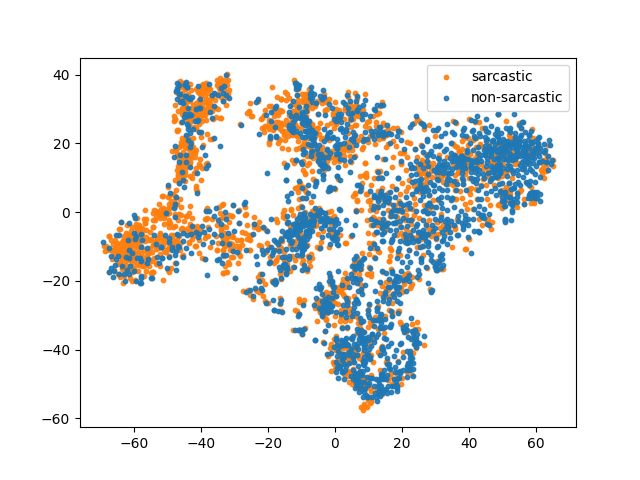
\includegraphics[width=\linewidth]{./figure/tsne_sarc_pol.png}
		 \subcaption{皮肉・非皮肉}
	\end{center}
%		\label{fig:40_tsne1-1}
	\end{minipage}
 	\begin{minipage}{0.4\hsize}
	\begin{center}
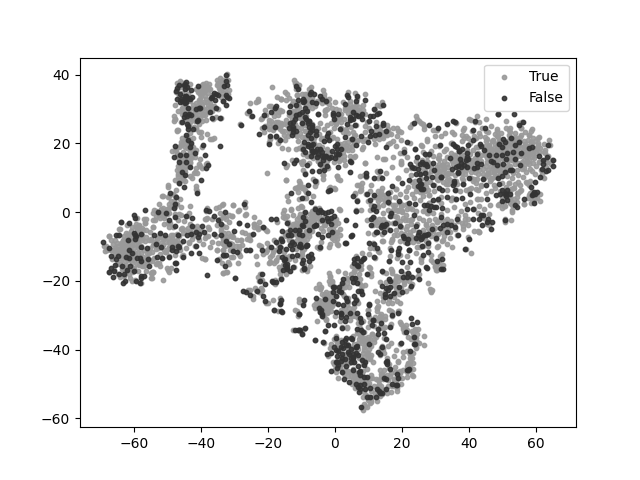
\includegraphics[width=\linewidth]{./figure/tsne_TorF_pol.png}
		\subcaption{正解・不正解}
 	 \end{center}
%		\label{fig:40_tsne1-2}
 	\end{minipage}
	\caption{t-SNE による可視化 (politics)}
	\label{fig:40_tsne1}
\end{center}
\end{figure}
% end figure

%%% figure minipage
\begin{figure}[tb]
\begin{center}
 	\begin{minipage}{0.4\hsize}
	\begin{center}
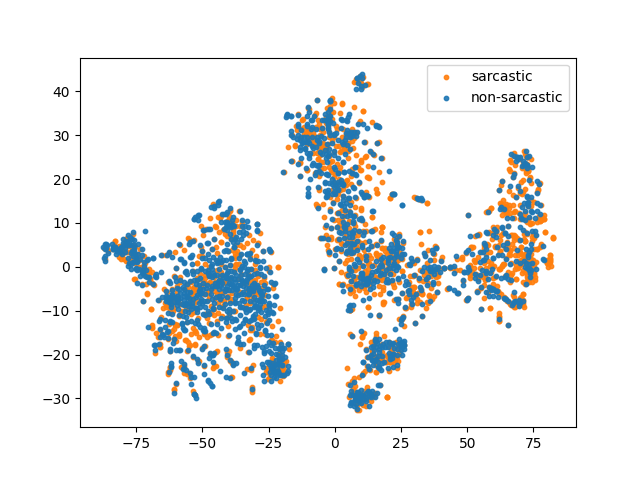
\includegraphics[width=\linewidth]{./figure/tsne_sarc_ask.png}
		 \subcaption{皮肉・非皮肉}
	\end{center}
%		\label{fig:40_tsne2-1}
	\end{minipage}
 	\begin{minipage}{0.4\hsize}
	\begin{center}
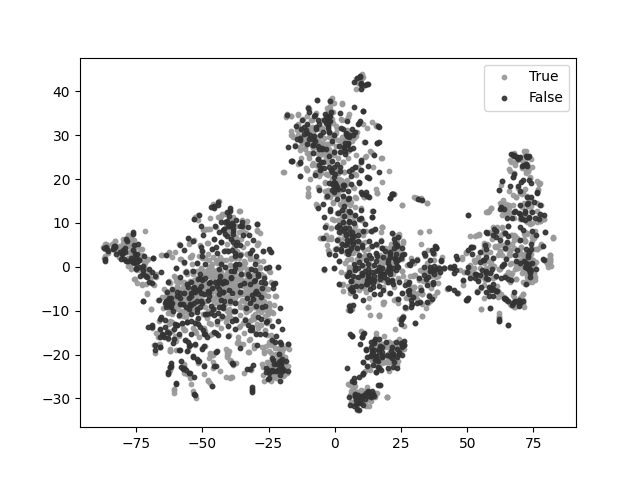
\includegraphics[width=\linewidth]{./figure/tsne_TorF_ask.png}
		\subcaption{正解・不正解}
 	 \end{center}
%		\label{fig:40_tsne2-2}
 	\end{minipage}
	\caption{t-SNE による可視化 (AskReddit)}
	\label{fig:40_tsne2}
\end{center}
\end{figure}
% end figure

%%% figure minipage
\begin{figure}[tb]
\begin{center}
 	\begin{minipage}{0.4\hsize}
	\begin{center}
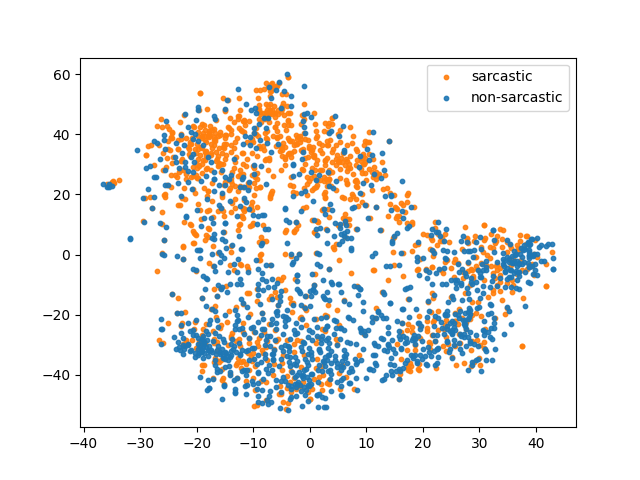
\includegraphics[width=\linewidth]{./figure/tsne_sarc_world.png}
		 \subcaption{皮肉・非皮肉}
	\end{center}
%		\label{fig:40_tsne3-1}
	\end{minipage}
 	\begin{minipage}{0.4\hsize}
	\begin{center}
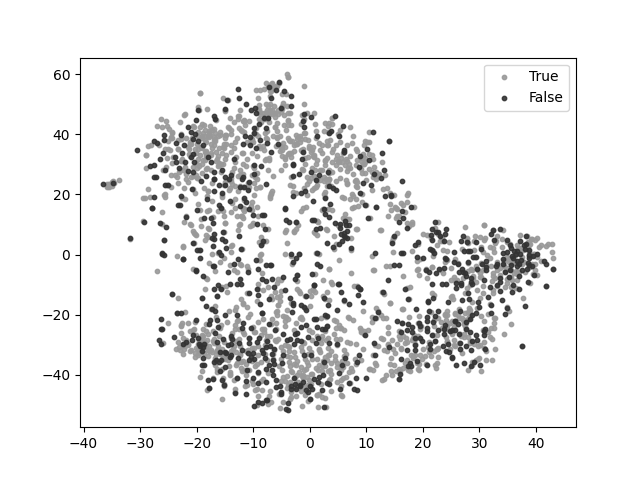
\includegraphics[width=\linewidth]{./figure/tsne_TorF_world.png}
		\subcaption{正解・不正解}
 	 \end{center}
%		\label{fig:40_tsne3-2}
 	\end{minipage}
	\caption{t-SNE による可視化 (worldnews)}
	\label{fig:40_tsne3}
\end{center}
\end{figure}
% end figure

%%% figure minipage
\begin{figure}[tb]
\begin{center}
 	\begin{minipage}{0.4\hsize}
	\begin{center}
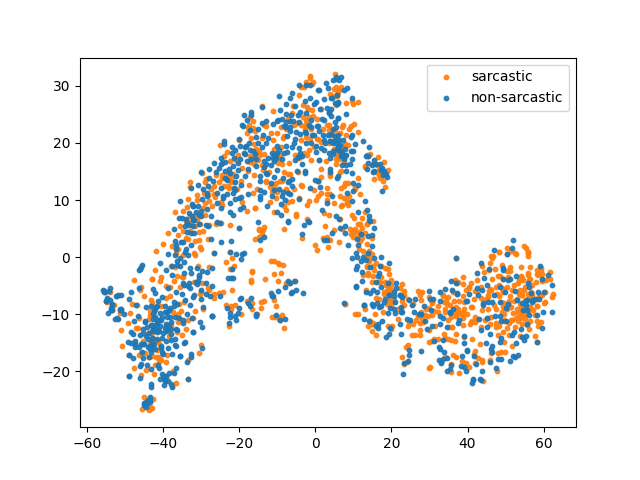
\includegraphics[width=\linewidth]{./figure/tsne_sarc_pc.png}
		 \subcaption{皮肉・非皮肉}
	\end{center}
%		\label{fig:40_tsne4-1}
	\end{minipage}
 	\begin{minipage}{0.4\hsize}
	\begin{center}
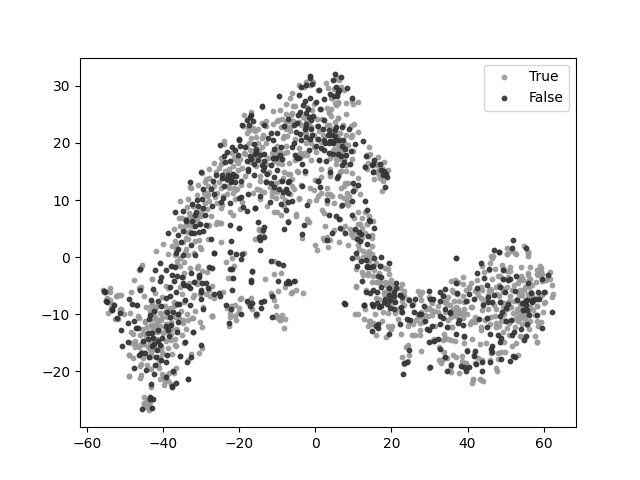
\includegraphics[width=\linewidth]{./figure/tsne_TorF_pc.png}
		\subcaption{正解・不正解}
 	 \end{center}
%		\label{fig:40_tsne4-2}
 	\end{minipage}
	\caption{t-SNE による可視化 (pcmasterrace)}
	\label{fig:40_tsne4}
\end{center}
\end{figure}
% end figure

%%% figure minipage
\begin{figure}[tb]
\begin{center}
 	\begin{minipage}{0.4\hsize}
	\begin{center}
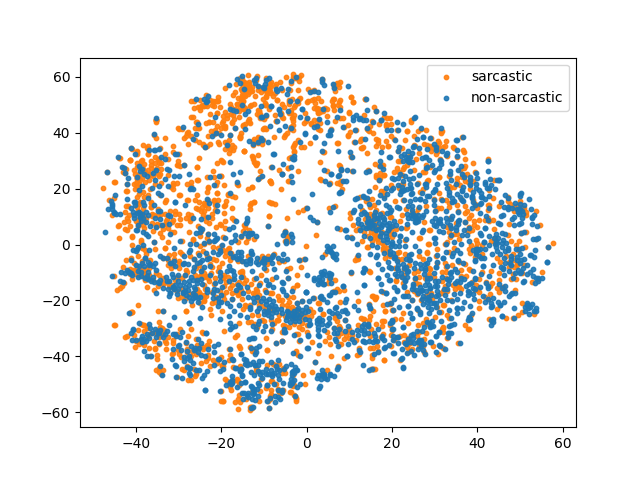
\includegraphics[width=\linewidth]{./figure/tsne_sarc_random.png}
		 \subcaption{皮肉・非皮肉}
	\end{center}
%		\label{fig:40_tsne4-1}
	\end{minipage}
 	\begin{minipage}{0.4\hsize}
	\begin{center}
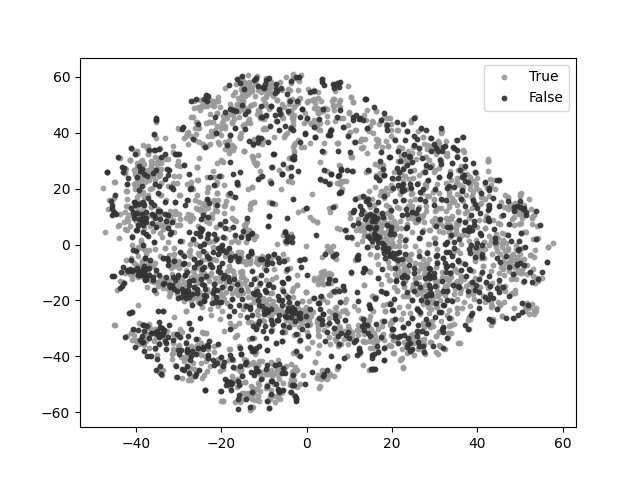
\includegraphics[width=\linewidth]{./figure/tsne_TorF_random.png}
		\subcaption{正解・不正解}
 	 \end{center}
%		\label{fig:40_tsne4-2}
 	\end{minipage}
	\caption{t-SNE による可視化 (random)}
	\label{fig:40_tsne5}
\end{center}
\end{figure}
% end figure


%%%%%%%%%%%%%%%%%%%%%%%%%%%%%%




